\documentclass{standalone}
\usepackage{tikz}
\usetikzlibrary{patterns, positioning}
\usepackage[sfdefault]{ClearSans} %% option 'sfdefault' activates Clear Sans as the default text font
\usepackage[T1]{fontenc}

\begin{document}
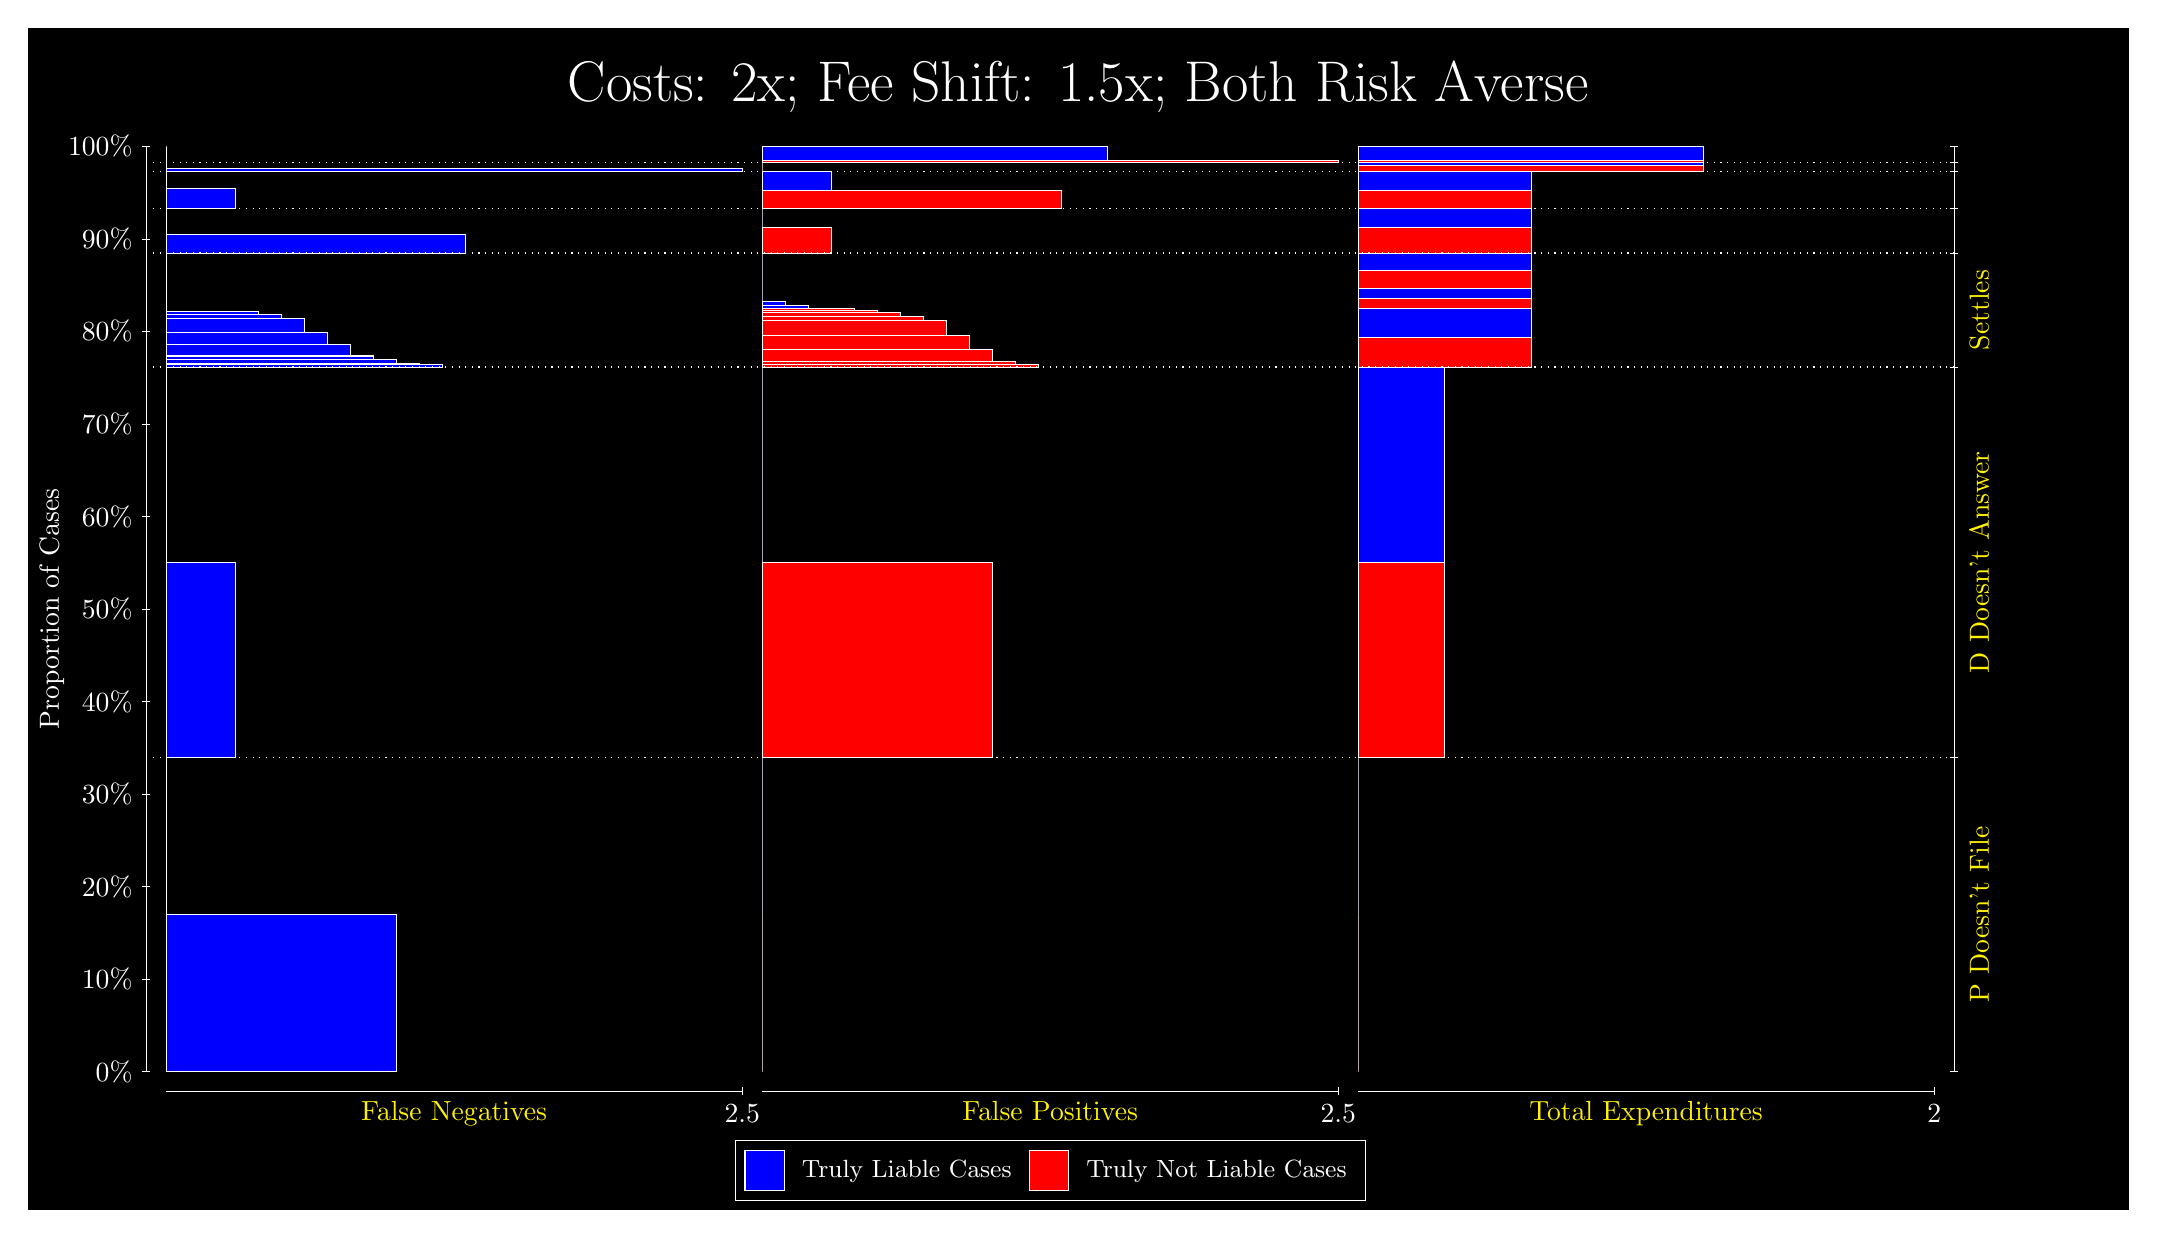
\begin{tikzpicture}
\draw[fill=black] (0,0) rectangle (26.667,15);
\draw[text=white] (0,13.5) rectangle (26.667,15) node[midway] {\huge Costs: 2x; Fee Shift: 1.5x; Both Risk Averse};
\draw[white, very thin] (1.5,1.75) -- (1.5,13.5);
\node[rotate=90, text=white, anchor=center] at (0.3, 7.625) {Proportion of Cases};
\draw[white, very thin] (1.45,1.75) -- (1.55,1.75);
\node[text=white, anchor=east] at (1.45, 1.75) {0\%};
\draw[white, very thin] (1.45,2.925) -- (1.55,2.925);
\node[text=white, anchor=east] at (1.45, 2.925) {10\%};
\draw[white, very thin] (1.45,4.1) -- (1.55,4.1);
\node[text=white, anchor=east] at (1.45, 4.1) {20\%};
\draw[white, very thin] (1.45,5.275) -- (1.55,5.275);
\node[text=white, anchor=east] at (1.45, 5.275) {30\%};
\draw[white, very thin] (1.45,6.45) -- (1.55,6.45);
\node[text=white, anchor=east] at (1.45, 6.45) {40\%};
\draw[white, very thin] (1.45,7.625) -- (1.55,7.625);
\node[text=white, anchor=east] at (1.45, 7.625) {50\%};
\draw[white, very thin] (1.45,8.8) -- (1.55,8.8);
\node[text=white, anchor=east] at (1.45, 8.8) {60\%};
\draw[white, very thin] (1.45,9.975) -- (1.55,9.975);
\node[text=white, anchor=east] at (1.45, 9.975) {70\%};
\draw[white, very thin] (1.45,11.15) -- (1.55,11.15);
\node[text=white, anchor=east] at (1.45, 11.15) {80\%};
\draw[white, very thin] (1.45,12.325) -- (1.55,12.325);
\node[text=white, anchor=east] at (1.45, 12.325) {90\%};
\draw[white, very thin] (1.45,13.5) -- (1.55,13.5);
\node[text=white, anchor=east] at (1.45, 13.5) {100\%};

\draw[white, very thin] (24.457,1.75) -- (24.457,13.5);
\draw[white, very thin] (24.407,1.75) -- (24.507,1.75);
\node[anchor=west] at (24.407, 1.75) {};
\draw[white, very thin] (24.407,5.7384) -- (24.507,5.7384);
\node[anchor=west] at (24.407, 5.7384) {};
\draw[white, very thin] (24.407,10.698) -- (24.507,10.698);
\node[anchor=west] at (24.407, 10.698) {};
\draw[white, very thin] (24.407,12.145) -- (24.507,12.145);
\node[anchor=west] at (24.407, 12.145) {};
\draw[white, very thin] (24.407,12.714) -- (24.507,12.714);
\node[anchor=west] at (24.407, 12.714) {};
\draw[white, very thin] (24.407,13.185) -- (24.507,13.185);
\node[anchor=west] at (24.407, 13.185) {};
\draw[white, very thin] (24.407,13.294) -- (24.507,13.294);
\node[anchor=west] at (24.407, 13.294) {};
\draw[white, very thin] (24.407,13.5) -- (24.507,13.5);
\node[anchor=west] at (24.407, 13.5) {};

\draw[white, very thin, fill=blue] (1.75,1.75) rectangle (4.6775,3.7442);
\draw[white, very thin, fill=red] (1.75,3.7442) rectangle (1.75,5.7384);
\draw[white, very thin, fill=blue] (1.75,5.7384) rectangle (2.6283,8.2182);
\draw[white, very thin, fill=red] (1.75,8.2182) rectangle (1.75,10.698);
\draw[white, very thin, fill=blue] (1.75,10.698) rectangle (5.2631,10.727);
\draw[white, very thin, fill=blue] (1.75,10.727) rectangle (4.9703,10.749);
\draw[white, very thin, fill=blue] (1.75,10.749) rectangle (4.6775,10.792);
\draw[white, very thin, fill=blue] (1.75,10.792) rectangle (4.3848,10.829);
\draw[white, very thin, fill=blue] (1.75,10.829) rectangle (4.3848,10.85);
\draw[white, very thin, fill=blue] (1.75,10.85) rectangle (4.092,10.986);
\draw[white, very thin, fill=blue] (1.75,10.986) rectangle (3.7993,11.141);
\draw[white, very thin, fill=blue] (1.75,11.141) rectangle (3.5065,11.313);
\draw[white, very thin, fill=blue] (1.75,11.313) rectangle (3.2138,11.362);
\draw[white, very thin, fill=blue] (1.75,11.362) rectangle (2.921,11.403);
\draw[white, very thin, fill=red] (1.75,11.403) rectangle (1.75,12.145);
\draw[white, very thin, fill=blue] (1.75,12.145) rectangle (5.5558,12.386);
\draw[white, very thin, fill=red] (1.75,12.386) rectangle (1.75,12.714);
\draw[white, very thin, fill=blue] (1.75,12.714) rectangle (2.6283,12.963);
\draw[white, very thin, fill=red] (1.75,12.963) rectangle (1.75,13.185);
\draw[white, very thin, fill=blue] (1.75,13.185) rectangle (9.0689,13.216);
\draw[white, very thin, fill=red] (1.75,13.216) rectangle (1.75,13.294);
\draw[white, very thin, fill=red] (1.75,13.294) rectangle (1.75,13.325);
\draw[white, very thin, fill=blue] (1.75,13.325) rectangle (1.75,13.5);
\draw[white, very thin, fill=red] (9.3189,1.75) rectangle (9.3189,3.7442);
\draw[white, very thin, fill=blue] (9.3189,3.7442) rectangle (9.3189,5.7384);
\draw[white, very thin, fill=red] (9.3189,5.7384) rectangle (12.246,8.2183);
\draw[white, very thin, fill=blue] (9.3189,8.2183) rectangle (9.3189,10.698);
\draw[white, very thin, fill=red] (9.3189,10.698) rectangle (12.832,10.728);
\draw[white, very thin, fill=red] (9.3189,10.728) rectangle (12.539,10.766);
\draw[white, very thin, fill=red] (9.3189,10.766) rectangle (12.246,10.927);
\draw[white, very thin, fill=red] (9.3189,10.927) rectangle (11.954,11.104);
\draw[white, very thin, fill=red] (9.3189,11.104) rectangle (11.661,11.286);
\draw[white, very thin, fill=red] (9.3189,11.286) rectangle (11.368,11.34);
\draw[white, very thin, fill=red] (9.3189,11.34) rectangle (11.075,11.389);
\draw[white, very thin, fill=red] (9.3189,11.389) rectangle (10.783,11.415);
\draw[white, very thin, fill=red] (9.3189,11.415) rectangle (10.49,11.44);
\draw[white, very thin, fill=blue] (9.3189,11.44) rectangle (9.9044,11.481);
\draw[white, very thin, fill=blue] (9.3189,11.481) rectangle (9.6116,11.53);
\draw[white, very thin, fill=blue] (9.3189,11.53) rectangle (9.3189,12.145);
\draw[white, very thin, fill=red] (9.3189,12.145) rectangle (10.197,12.473);
\draw[white, very thin, fill=blue] (9.3189,12.473) rectangle (9.3189,12.714);
\draw[white, very thin, fill=red] (9.3189,12.714) rectangle (13.125,12.936);
\draw[white, very thin, fill=blue] (9.3189,12.936) rectangle (10.197,13.185);
\draw[white, very thin, fill=red] (9.3189,13.185) rectangle (9.3189,13.264);
\draw[white, very thin, fill=blue] (9.3189,13.264) rectangle (9.3189,13.294);
\draw[white, very thin, fill=red] (9.3189,13.294) rectangle (16.638,13.325);
\draw[white, very thin, fill=blue] (9.3189,13.325) rectangle (13.71,13.5);
\draw[white, very thin, fill=red] (16.888,1.75) rectangle (16.888,3.7442);
\draw[white, very thin, fill=blue] (16.888,3.7442) rectangle (16.888,5.7384);
\draw[white, very thin, fill=red] (16.888,5.7384) rectangle (17.986,8.2183);
\draw[white, very thin, fill=blue] (16.888,8.2183) rectangle (17.986,10.698);
\draw[white, very thin, fill=red] (16.888,10.698) rectangle (19.083,11.08);
\draw[white, very thin, fill=blue] (16.888,11.08) rectangle (19.083,11.437);
\draw[white, very thin, fill=red] (16.888,11.437) rectangle (19.083,11.566);
\draw[white, very thin, fill=blue] (16.888,11.566) rectangle (19.083,11.697);
\draw[white, very thin, fill=red] (16.888,11.697) rectangle (19.083,11.928);
\draw[white, very thin, fill=blue] (16.888,11.928) rectangle (19.083,12.145);
\draw[white, very thin, fill=red] (16.888,12.145) rectangle (19.083,12.473);
\draw[white, very thin, fill=blue] (16.888,12.473) rectangle (19.083,12.714);
\draw[white, very thin, fill=red] (16.888,12.714) rectangle (19.083,12.936);
\draw[white, very thin, fill=blue] (16.888,12.936) rectangle (19.083,13.185);
\draw[white, very thin, fill=red] (16.888,13.185) rectangle (21.279,13.264);
\draw[white, very thin, fill=blue] (16.888,13.264) rectangle (21.279,13.294);
\draw[white, very thin, fill=red] (16.888,13.294) rectangle (21.279,13.325);
\draw[white, very thin, fill=blue] (16.888,13.325) rectangle (21.279,13.5);
\draw[white, dotted] (1.5,5.7384) -- (24.457,5.7384);
\draw[white, dotted] (1.5,10.698) -- (24.457,10.698);
\draw[white, dotted] (1.5,12.145) -- (24.457,12.145);
\draw[white, dotted] (1.5,12.714) -- (24.457,12.714);
\draw[white, dotted] (1.5,13.185) -- (24.457,13.185);
\draw[white, dotted] (1.5,13.294) -- (24.457,13.294);
\draw[white, very thin] (1.75,1.5) -- (9.0689,1.5);
\node[text=yellow, anchor=north] at (5.4094, 1.5) {False Negatives};
\draw[white, very thin] (9.0689,1.45) -- (9.0689,1.55);
\node[text=white, anchor=north] at (9.0689, 1.45) {2.5};

\draw[white, very thin] (9.3189,1.5) -- (16.638,1.5);
\node[text=yellow, anchor=north] at (12.978, 1.5) {False Positives};
\draw[white, very thin] (16.638,1.45) -- (16.638,1.55);
\node[text=white, anchor=north] at (16.638, 1.45) {2.5};

\draw[white, very thin] (16.888,1.5) -- (24.207,1.5);
\node[text=yellow, anchor=north] at (20.547, 1.5) {Total Expenditures};
\draw[white, very thin] (24.207,1.45) -- (24.207,1.55);
\node[text=white, anchor=north] at (24.207, 1.45) {2};

\node[text=yellow, centered, rotate=90] at (24.777, 3.7442) {P Doesn't File};
\node[text=yellow, centered, rotate=90] at (24.777, 8.2183) {D Doesn't Answer};
\node[text=yellow, centered, rotate=90] at (24.777, 11.421) {Settles};





\draw (12.978300999999998,1.5) node[draw=none] (baseCoordinate) {};
\begin{scope}[align=center]
        \matrix[scale=0.5, draw=white, below=0.5cm of baseCoordinate, nodes={draw}, column sep=0.1cm]{
            \node[rectangle, draw, minimum width=0.5cm, minimum height=0.5cm, fill=blue] {}; &
            \node[draw=none, font=\small, text=white] (B) {Truly Liable Cases}; &
            \node[rectangle, draw, minimum width=0.5cm, minimum height=0.5cm, fill=red] {}; &
            \node[draw=none, font=\small, text=white] (B) {Truly Not Liable Cases}; \\
            };
\end{scope}

\end{tikzpicture}
\end{document}